% preamble and style file for M&R lecture slides
\documentclass[11.5pt,sans,english]{beamer}

\usetheme{EastLansing}
\usecolortheme{lily}

\usepackage[most]{tcolorbox}

\usepackage{verbatim}
%\usepackage{ulem}
%\usepackage{fontawesome}
%\usepackage{tikz}
%\usepackage{pifont}
%\usepackage{tabularx}
\usepackage{array,booktabs,xcolor,colortbl,multirow,rotating,amssymb}
%\usepackage{amsmath}
% \usepackage{vwcol}
% \usepackage[T1]{fontenc}

  
\newcommand\vect[1]{\underline{\mathbf{#1}}}
\newcommand\unitvect[1]{\hat{\boldsymbol{#1}}}
%\newcommand\hatdot[1] { \hat{ \dot{ \boldsymbol{#1} } } }

\newtcbox
{\keyc}{on line,arc=2pt, colback=yellow!30!white, colframe=yellow!30!black, before upper={\rule[-3pt]{0pt}{10pt} },boxrule=1pt,boxsep=0pt,left=6pt,right=6pt,top=2pt,bottom=2pt,}

\newtcbox
{\keyb}{on line,arc=1pt, colback=blue!30!white, colframe=blue!30!black, before upper={\rule[-3pt]{0pt}{10pt} },boxrule=1pt,boxsep=0pt,left=6pt,right=6pt,top=2pt,bottom=2pt,}

\newtcbox
{\keyl}{on line,arc=1pt, colback=pink!30!white, colframe=blue!30!black, before upper={\rule[-3pt]{0pt}{10pt} },boxrule=1pt,boxsep=0pt,left=6pt,right=6pt,top=2pt,bottom=2pt,}

\newtcbox
{\keyw}{on line,arc=1pt, colback=red!30!white, colframe=blue!30!black, before upper={\rule[-3pt]{0pt}{10pt} },boxrule=1pt,boxsep=0pt,left=6pt,right=6pt,top=2pt,bottom=2pt,}

\newtcbox
{\keya}{on line,arc=1pt, colback=purple!30!white, colframe=blue!30!black, before upper={\rule[-3pt]{0pt}{10pt} },boxrule=1pt,boxsep=0pt,left=6pt,right=6pt,top=2pt,bottom=2pt,}

\newtcbox[auto counter,number within=section]
{keyf}
{
enhanced,
on line,
  boxsep=0pt,
  left=6pt,right=6pt,top=2pt,bottom=2pt,
  arc=5pt,
  boxrule=1pt,
  rightrule=38pt,
colback=green!10!white, 
colframe=green!50!black, 
title=\thetcbcounter,
detach title,
overlay unbroken and first ={
    \node[%rotate=90,
          %minimum width=1cm,
          anchor=south,
          font=\sffamily\bfseries\tiny,
          %yshift=-10pt,
          yshift=-5pt,
          xshift=-20pt,
          white]
    at (frame.east) {\thetcbcounter};
  }
}


\usepackage{xcolor}

%\usepackage{hyperref}
%\hypersetup{
%  pdfauthor={Lily Asquith},
%  urlcolor=blue,
%  colorlinks=true,
%  linkcolor=blue,
%  bookmarks=true
%}

%---------------------------------------------%
%              LILY'S COLOURS           %
%---------------------------------------------%
\definecolor{Wash}{RGB}{204,204,204}
%\definecolor{Pinky}{RGB}{254,200,254}%violet
\definecolor{Pinky}{RGB}{219,	240,	253}%violet
\definecolor{Bluey}{RGB}{0,190,255}%deep sky blue
\definecolor{DarkGrey}{RGB}{28,66,137}%dar grey
\definecolor{SussexWhite}{RGB}{253,255,254}%dar grey
\definecolor{LightGray}{RGB}{184,184,255}
\definecolor{YesGreen}{RGB}{0,128,0}
\definecolor{NoRed}{RGB}{250,0,0}



\definecolor{myred}{RGB}{255,153,153}
\definecolor{myorange}{RGB}{255,204,153}
\definecolor{myyellow}{RGB}{255,255,153}
\definecolor{mygreen}{RGB}{153,255,153}
\definecolor{mycyan}{RGB}{153,255,255}
\definecolor{myblue}{RGB}{153,204,255}
\definecolor{myviolet}{RGB}{153,153,255}
\definecolor{mypurple}{RGB}{204,153,255}
\definecolor{mypink}{RGB}{255,204,255}
\definecolor{mycoral}{RGB}{255,153,204}

%-----------------------------------------------------%
%              LILY'S COLUMN TYPES          %
%-----------------------------------------------------%
\newcolumntype{a}{>{\raggedright\arraybackslash}l}	
\newcolumntype{q}{>{\raggedright\arraybackslash}m{8cm}} 

%--------------------------------------------%
%              LILY'S SYMBOLS          %
%--------------------------------------------%
\newcommand{\dfinger}{\large{\textcolor{black}{\ding{43}}}\scriptsize}
\newcommand{\dstar}{\large{\textcolor{black}{\ding{76}}}\scriptsize}
\newcommand{\dwrite}{\large{\textcolor{black}{\ding{45}}}\scriptsize}
\newcommand{\ddiamond}{\small{\textcolor{DarkGrey}{\ding{117}}}\scriptsize}
\newcommand{\ddiamondwhite}{\small{\textcolor{SussexWhite}{\ding{117}}}\scriptsize}
\newcommand{\experiment}{\small{\textcolor{magenta}{\faCogs }}\scriptsize}
\newcommand{\watchit}{\textcolor{blue}{ \faYoutube}}


\makeatletter
\newcommand\notsotiny{\@setfontsize\notsotiny{6.5}{7.5}}
\makeatother


% 
\title[ Mechanics \& Relativity]{Mechanics \& Relativity}
%\subtitle{\textbf{Topic 1: Kinematics }}
\author[Dr Lily Asquith (Lily)]{ Dr Lily Asquith (Lily)}
\date[Week 5]{Week 5}
\logo{

\includegraphics[width=1.5cm]{../../utils/uslogo.jpg}
}


\begin{document}


\begin{frame}
\titlepage
\end{frame} 


%\begin{frame}
%Please load pollev/ilovephysics
%\end{frame}
%
%\section{M\&R 5: Forces 2}
%\begin{frame}
%\frametitle{Forces 2} 
%\normalsize
%
%This week's topics:\\[3ex]
%
%\begin{itemize}
%\item[5.1] Friction \& Drag\\[3ex]
%\item[5.2] Springs\\[3ex]
%\item[5.3] Problem Solving\\[3ex]
%\end{itemize}
%\end{frame} 
% 
%
% \subsection{Friction}
%
%\begin{frame}{Friction}
%\small
%
%Frictional forces are responsive. \\[1ex]
%There are two kinds of frictional force: static and kinetic.\\[1ex]
%Kinetic friction only applies when there is sliding.\\[1ex]
%$F_{\mu_s} \leq \mu_s N$\\[1ex]
%$F_{\mu_k} = \mu_k N$\\[1ex]
%
%Often, friction problems come down to figuring out the normal force.
%
%\end{frame}
%
%
%\begin{frame}{What has friction got to do with the normal force?}
%
%
%\small
%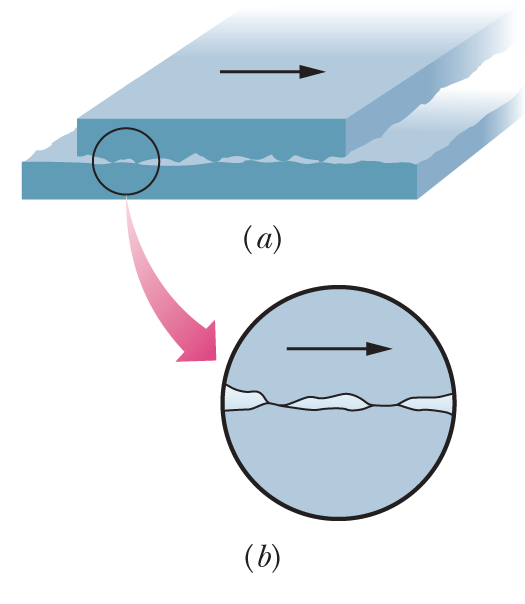
\includegraphics[scale=0.8]{fric-micro}
%
%\end{frame}
%
%
%
%
%
%
%\begin{frame}{Friction 1: Will it move?}
%\small
%A 1kg wooden crate is on a horizontal surface with $\mu_s = 0.3$. What is its acceleration if I apply a horizontal force of magnitude 10N?\\[1ex]
%\vspace{10cm}
%
%\end{frame}
%
%
%
%\begin{frame}{Friction 1: Will it move?}
%\small
%A wooden crate is on an inclined plane with $\mu_s = 0.4$. At what angle of incline will it begin to slide down the plane?\\[1ex]
%\vspace{10cm}
%
%\end{frame}
%
%
%\begin{frame}{Friction 1: Will it move?}
%\small
%The same wooden crate is now being pinned to a wall with $\mu_s =0.5$ by a horizontal force of unknown magnitude. What is the minimum magnitude of this force to prevent the crate sliding down the wall?\\[1ex]
%\vspace{10cm}
%
%
%\end{frame}
%
%\begin{frame}{The two frictional forces}
%\small
%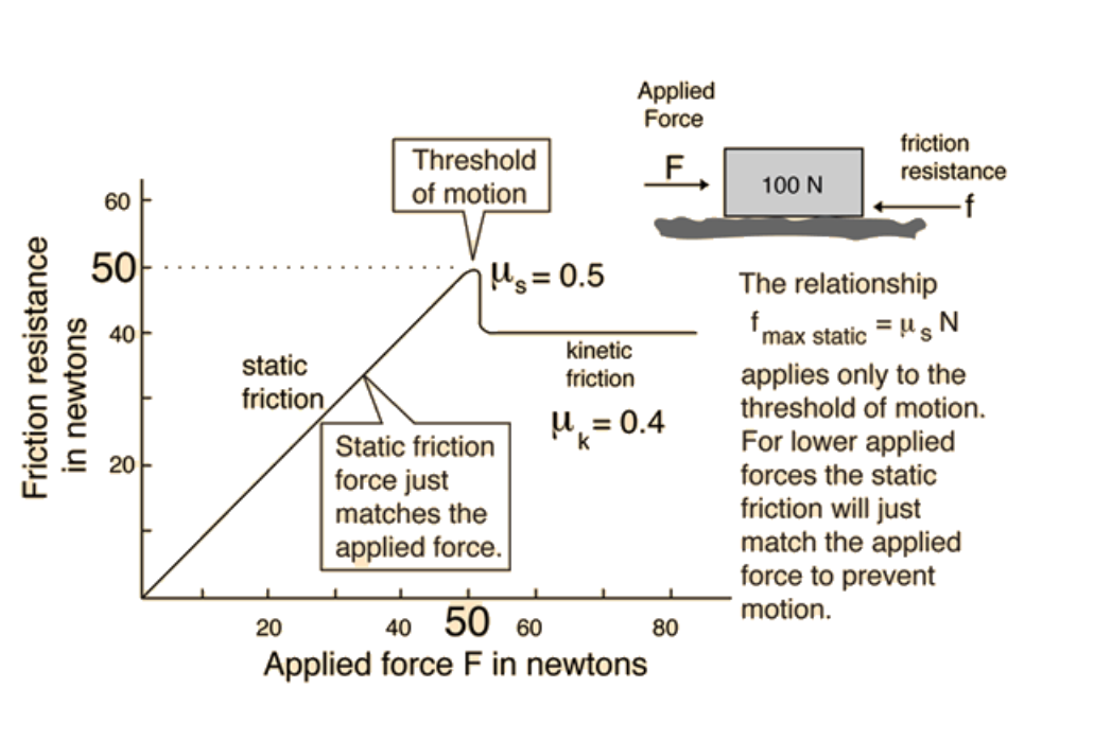
\includegraphics[scale=0.6]{friction}
%
%\end{frame}
%
%
%
%\begin{frame}{Friction 2: Sliding}
%\small
%A 200 kg car is driving along a wet road at  90 km/hr when it starts to slide out of control. If the car comes to a stop in 300m, what is $\mu_{k}$? Is this possible?\\
%\vspace{10cm}
%
%
%\end{frame}
%
%
%
% \subsection{Drag}
%
%
%\begin{frame}{Drag}
%\Huge
%\begin{center}
%$F_{D} = \frac{1}{2} C_{D} \rho A v^2$
%\end{center}
%\small
%
%\end{frame}
%
%
%\begin{frame}{Terminal Velocity}
%\small
%
%\end{frame}



% LECTURE 2
 \subsection{Kinetic Energy}


\begin{frame}{Work done by a force}
\small
The work done by a force is $W=\int F\cdot ds$
\vspace{10cm}
\end{frame}

\begin{frame}{Kinetic Energy}
\small
The change in an objects KE is equal to the work done on that object by some external force.\\
\vspace{10cm}
\end{frame}

 \subsection{Springs}

\begin{frame}{Springs}
\small
Springs are a special situation because of the way they respond to external forces\\[1ex]

Hooke's law: $F_{x} = -kx$\\[1ex]

The equilibirium (relaxed) state of a spring corresponds to $x=0$.\\

If I exten


\vspace{10cm}
\end{frame}
%
% \subsection{Problems}
%
%
%\begin{frame}{Problems}
%\small
%
%\vspace{10cm}
%\end{frame}

\end{document}